\section{Problem Formulation}
\label{sec:formulation}

We formalize trustworthy phishing detection as \emph{selective prediction over a
grounded evidence-agreement score}: rather than always emitting a label, the detector
acts only when its evidence is both agreed-upon and verified, and otherwise abstains.
We proceed in five steps -- what the detector observes (\autoref{sec:form-prelim}),
the score it computes (\autoref{sec:form-gea}), the act/abstain objective it optimizes
(\autoref{sec:form-objective}), the requirements the method must meet
(\autoref{sec:form-req}), and the resulting framework (\autoref{sec:form-overview}).
\autoref{tab:notation} collects the notation.

\subsection{Preliminaries}
\label{sec:form-prelim}

\sstitle{Setting}
A detector receives a webpage $\page$ -- represented by its URL, DOM, rendered
screenshot, and, where the capture provides them, the Transport Layer Security
(TLS) certificate and redirect chain -- and must decide whether $\page$ is
phishing. The last two are part of the schema for generality; on the corpus used
in \autoref{sec:experiments} they are absent and the corresponding cue types are
inert there. It has access to two resources. The first is a panel
$\panel=\{m_1,\dots,m_M\}$ of $M$ \emph{diverse} LLM \emph{evidence agents}: they come
from different model families and include at least one vision-language model that reads
the screenshot, and each can call a set of verification \emph{tools} that re-derive
factual signals from $\page$. The second is a fixed, typed \emph{evidence schema}
$\Uschema$ that fixes the vocabulary of facts the agents may cite. A \emph{cue}
$u=(t,v)\in\Uschema$ pairs a type $t$ (e.g.\ \textsf{form-action-domain},
\textsf{cert-org}, \textsf{redirect-target}, \textsf{logo-brand},
\textsf{credential-intent}) with a value $v$ (e.g.\ the domain a login form posts to);
every type has a corresponding tool $\gver$ that re-derives it from $\page$, which is
what makes a cue checkable rather than merely asserted.

\sstitle{Agent outputs and the shared cue set}
Run on $\page$, each agent investigates the page and returns a verdict together with
the cues it grounds through tool calls:
\begin{equation}
m_i(\page) = \bigl(y_i(\page),\ \evset_i(\page)\bigr),\quad
y_i\in\{\textsf{phish},\textsf{benign}\},\ \evset_i\subseteq\Uschema .
\label{eq:output}
\end{equation}
Pooling the agents' cited cues gives the page's \emph{shared cue set}
$\bigcup_i\evset_i(\page)$, the universe of evidence anyone raised, and the verdict is
the majority vote $\hat y(\page)=\mathrm{maj}_i\,y_i(\page)$. Within the shared set, a
\emph{consensus} cue is one that a strict majority of the agents assert with a
consistent value, $\cons(\page)=\{u: \lvert\{i: u\in\evset_i\}\rvert > M/2\}$ -- the
evidence the panel independently corroborates; these consensus cues are the evidence
\toolname{} trusts to drive the verdict and returns as the explanation.
\begin{table}[!h]
\caption{Summary of important notations.}
\label{tab:notation}
\footnotesize
\setlength{\tabcolsep}{4pt}
\begin{tabularx}{\columnwidth}{l >{\raggedright\arraybackslash}X}
\toprule
Symbol & Meaning \\
\midrule
$\page$                 & a webpage under test (URL, DOM, screenshot, cert, redirects) \\
$\panel=\{m_1,\dots,m_M\}$ & panel of $M$ diverse LLM evidence agents ($M{=}3$) \\
$\Uschema$              & fixed typed evidence-cue schema (\S\ref{sec:elicit}) \\
$\evset_i\subseteq\Uschema$ & grounded cues agent $m_i$ cites on $\page$ \\
$\cons$                 & \emph{consensus} cue set (cues a majority of agents assert) \\
$\gver(u,\page)\in[0,1]$ & tool that re-derives cue $u$'s type from $\page$ \\
$\agr(\page)\in[0,1]$   & evidence-level agreement over the shared cue set \\
$\grd(\page)\in[0,1]$   & groundedness of the consensus cues \\
$\geascore(\page)=\agr\!\cdot\!\grd$ & Grounded Evidence-Agreement score \\
$\thr$                  & abstention threshold (acts iff $\geascore\ge\thr$) \\
$\hat\rho=\kappa(\geascore)$ & calibrated map $\geascore\!\to\!\Prob(\text{correct})$, fit on a labeled split \\
\bottomrule
\end{tabularx}
\end{table}


\subsection{Grounded Evidence-Agreement}
\label{sec:form-gea}
Existing detectors estimate per-verdict reliability from the \emph{label} channel
alone -- a single model's confidence, or the concordance of the verdicts
$\{y_i\}$~\cite{guo2017calibration,ensembleornot2024,dawid1979maximum}. The flaw is
that the label channel is blind to \emph{why} the agents agree. We instead score the
\emph{evidence} channel with two complementary factors: how much of the cited evidence
the panel agrees on, and how much of that agreed evidence the page actually bears out.
Formally, the evidence-level agreement and the groundedness of the consensus are
\begin{align}
\agr(\page) &= \frac{\lvert \cons(\page)\rvert}
                    {\bigl\lvert \bigcup_i \evset_i(\page)\bigr\rvert},
\label{eq:agree}\\[2pt]
\grd(\page) &= \frac{1}{\lvert \cons(\page)\rvert}
               \sum_{u\in \cons(\page)} \gver(u,\page),
\label{eq:ground}
\end{align}
where $\gver(u,\page)\in[0,1]$ is the tool that re-derives cue $u$'s type from $\page$
(deterministic, returning $0$ or $1$, for \textsf{form-action}, \textsf{cert-org}, and
\textsf{redirect}; perceptual, returning a similarity, for \textsf{logo-brand}), and we
set $\grd(\page)\!=\!0$ when $\cons(\page)$ is empty. Thus $\agr$ rises only as the
agents converge on the \emph{same} cues, and $\grd$ rises only as those agreed cues
survive re-derivation from the page. The \emph{Grounded Evidence-Agreement} score is
their product,
\begin{equation}
\geascore(\page) = \agr(\page)\cdot\grd(\page)\in[0,1].
\label{eq:gea}
\end{equation}
The product, rather than a sum or average, is deliberate: either failure alone drives
$\geascore$ to zero. Agreement on cues the page does not confirm sends
$\grd\!\to\!0$, and a panel that concurs on the label while citing disjoint cues sends
$\agr\!\to\!0$; only when the agents agree on the evidence \emph{and} the page bears it
out does $\geascore$ stay high. This is exactly the conjunction the label channel
cannot express. On a clean corpus the two factors are largely redundant -- agents that
converge on a cue usually converge on one the page bears out, so $\agr$ and $\grd$ are
strongly correlated (Pearson $0.71$ on our test split, with only $0.4\%$ of
high-agreement pages poorly grounded) and either factor would rank pages similarly. The
product earns its keep precisely when the two \emph{decouple}: when evidence is corrupted
-- a morphed logo, a cloaked form action -- agents may still agree on a cue the page no
longer carries, driving $\grd$ (and thus $\geascore$) down while $\agr$ stays high. We
exercise this regime directly in \autoref{sec:exp_adv}.

\subsection{Selective Objective}
\label{sec:form-objective}
\toolname{} is a \emph{selective} detector: it acts with the verdict $\hat y(\page)$
when $\geascore(\page)\ge\thr$ for a threshold $\thr$, and otherwise abstains, emitting
$\bot$ to escalate the page. A threshold induces two quantities -- the \emph{coverage}
$\phi(\thr)$, the fraction of pages on which the detector acts, and the \emph{selective
risk} $r(\thr)$, the error rate on exactly those pages:
\begin{equation}
\phi(\thr)=\Prob[\geascore\ge\thr],\quad
r(\thr)=\Prob\bigl[\hat y\neq y \,\big|\, \geascore\ge\thr\bigr],
\label{eq:objective}
\end{equation}
with $y$ the true label. Sweeping $\thr$ traces the risk--coverage curve $r(\phi)$,
and a good score keeps this curve low everywhere -- equivalently, it minimizes the area
under it (AURC). To turn the raw score into an actionable threshold, we fit a
calibrator $\kappa:\geascore\mapsto\hat\Prob(\hat y=y)$ on a held-out labeled split
that maps the score to a probability of being correct, and pick the operating point
$\thr$ that realizes a target risk. The per-page \emph{output} is then a verdict or an
abstention, the calibrated trust $\hat\rho=\kappa(\geascore)$, and, when acting, the
consensus cue set $\cons(\page)$ as the explanation.

\subsection{Design Requirements}
\label{sec:form-req}
Scoring the evidence channel rather than the label channel imposes three requirements,
each repairing one limitation of label-centric reliability identified in
\autoref{sec:intro}. The framework (\autoref{sec:form-overview}) discharges each
through a named component, and \autoref{sec:experiments} measures its effect.
\begin{compactitem}
\item[(\req{1})] \emph{Emit structured, checkable evidence.} The label channel returns
no auditable artifact, only the verdict $\hat y$, so an action cannot be justified or
verified (answers \limit{1}; realized by agentic evidence elicitation, component $C_1$,
\autoref{sec:elicit}, and returned as the explanation throughout).
\item[(\req{2})] \emph{Measure agreement at the evidence level.} Concordance read from
the verdicts $\{y_i\}$ cannot distinguish a panel that agrees \emph{because} the page
carries the evidence from one that agrees on the label while resting on entirely
different cues (answers \limit{2}; realized by evidence agreement $\agr$, component
$C_2$, \autoref{sec:agree}; ablated in \autoref{sec:exp_rq3}).
\item[(\req{3})] \emph{Ground cited evidence to the page.} Evidence the panel cites in
agreement may still be a \emph{shared} hallucination, which agreement alone would
reward; it must instead be checked against $\page$ (answers \limit{3}; realized by
tool-grounding $\grd$, component $C_3$, \autoref{sec:ground}; ablated in
\autoref{sec:exp_rq3}).
\end{compactitem}
This limitation--requirement--component thread runs through the paper: each $C_i$ is
developed in \autoref{sec:method} and isolated by an ablation row in
\autoref{sec:exp_rq3}, so the contribution of every requirement is measured, not
assumed.

\subsection{Framework Overview}
\label{sec:form-overview}
\begin{figure*}[!h]
\centering
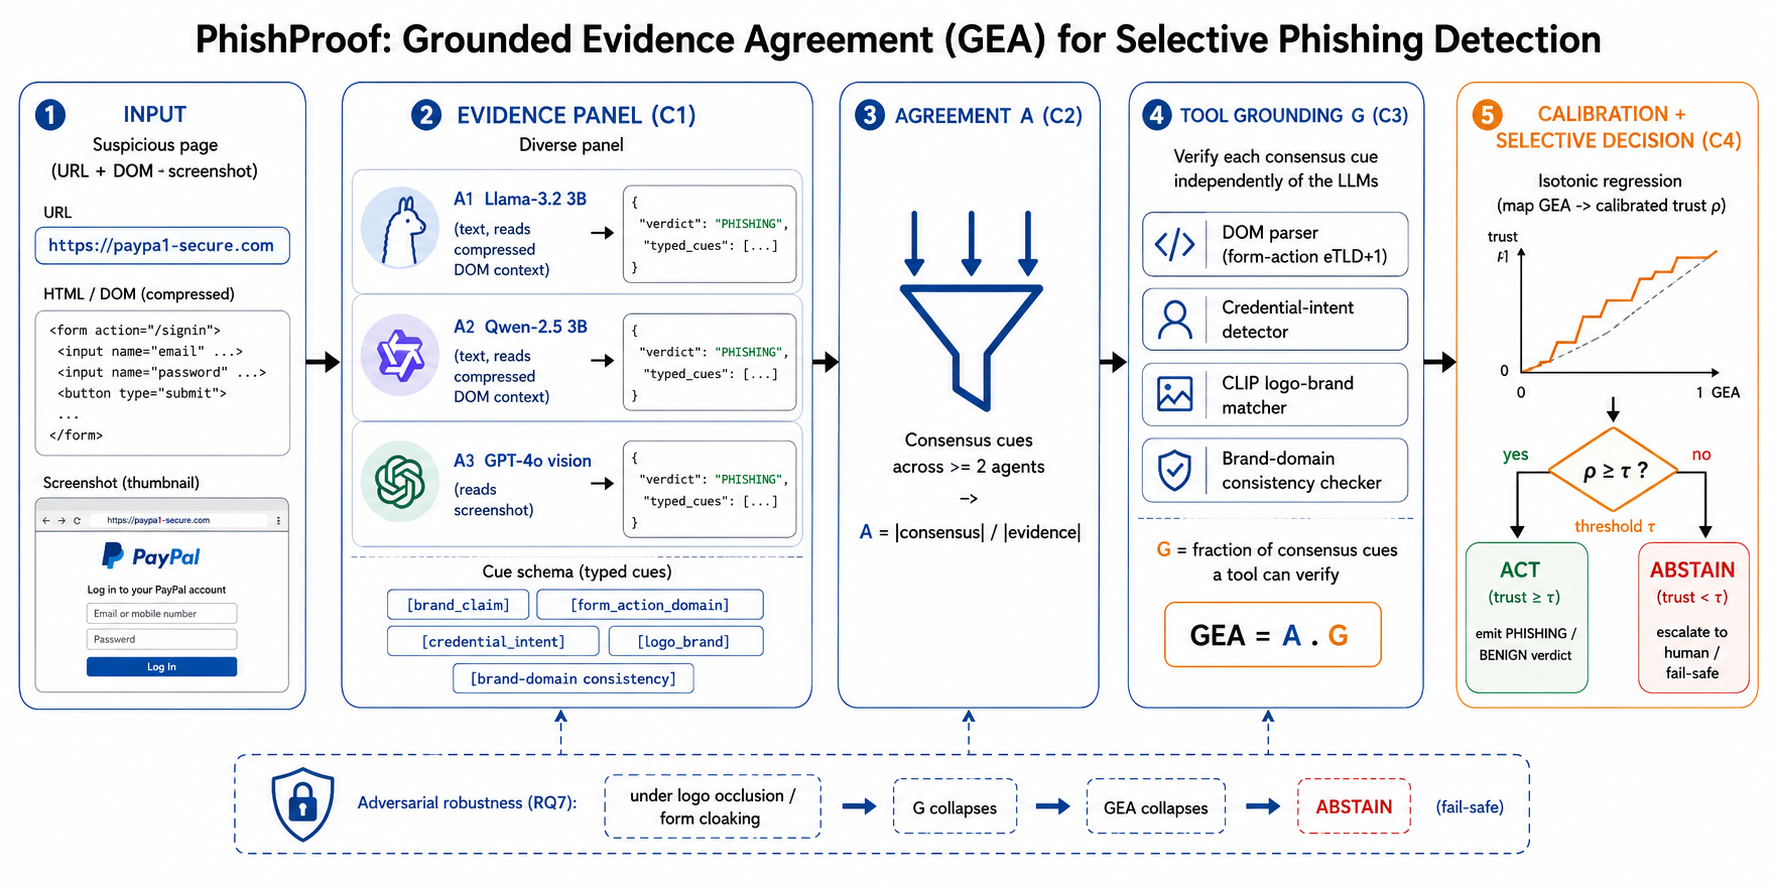
\includegraphics[width=\textwidth]{../figures/fig_overview_visual.png}
\caption{\toolname{} qualitative pipeline. Agents inspect the same page from
complementary views and cite typed evidence cues into a shared set. The system
trusts a verdict only when the agents converge on the same cues and the tool bank
can re-check those cues against the live page. The calibrated selector returns the
label with the verified cues when the evidence is shared and grounded; otherwise it
abstains, including cases where the label vote is plausible but the reasons are thin
or unverified. The threshold and calibrator are set on a held-out labeled split.}
\Description{A four-stage qualitative pipeline. The first panel shows a suspicious
login page and three agents emitting typed evidence cues. The second panel shows a
shared set of typed cues with provenance pins and a highlighted consensus
(agreement A). The third panel shows DOM, brand, consistency, and logo tools re-checking
each consensus cue into a groundedness score G. The final panel forms GEA = A times
G, calibrates it to a probability of correctness on a held-out labeled split, and
acts above a threshold by returning the verified cues or abstains otherwise.}
\label{fig:overview}
\end{figure*}
End-to-end, \toolname{} turns a page into a trusted-and-explained verdict in four
steps, drawn in \autoref{fig:overview} and developed one per subsection in
\autoref{sec:method}; the four components $C_1$--$C_4$ map one-to-one onto these steps.
\textbf{(1)~Investigate.} Each agent plans which signals to examine and calls the
verification tools, emitting its verdict and a set of typed, tool-checkable cues into
the shared cue set ($C_1$ agentic evidence elicitation, \req{1},
\autoref{sec:elicit}).
\textbf{(2)~Aggregate on evidence.} Over the shared set we form the strict-majority
consensus and measure how much of the cited evidence falls within it -- the
evidence-level agreement $\agr$ -- instead of counting how often the verdicts concur
($C_2$, \req{2}, \autoref{sec:agree}).
\textbf{(3)~Verify against the page.} Each consensus cue is re-derived by its tool, and
the groundedness $\grd$ discounts any consensus that the page does not actually bear
out, catching shared hallucinations ($C_3$, \req{3}, \autoref{sec:ground}).
\textbf{(4)~Decide and explain.} The score $\geascore=\agr\cdot\grd$ is calibrated on a
labeled split and thresholded into an act/abstain decision; when it acts it returns the
consensus cues as the explanation, and otherwise escalates the page ($C_4$ calibrated
selection, \autoref{sec:select}). Because the score is a product, a verdict survives to
action only when steps~(2) and~(3) both hold -- precisely guarding against the
right-label/wrong-reason and shared-hallucination failures the label channel misses.
